\section{Nested Arrays}
 The array elements are ordered in memory in row-major order, meaning all elements of row 0, which can be written A[0], followed by all elements of row 1 (A[1]), and so on. In other words, since the memory is one dimensional, nested arrays in C programming language are saved in a \textit{row-major} order in the memory. Figure~\ref{fig:nested-array} demonstrates how 2-D array \texttt{arr[3][4]} is saved in the memory in a row-major order.

 
 If an array is declared as:
\[
\text{Type } A[R][C];
\]
where \textit{Type} can be \texttt{char}, \texttt{int}, \texttt{long}, etc., the \textbf{memory address} of an element \( A[i][j] \) in a row-major order layout is calculated as:

\begin{equation}
A[i][j] = A + \text{sizeof}(\text{Type}) \times (C \times i + j)
\end{equation}

\begin{figure}[t]
    \centering
    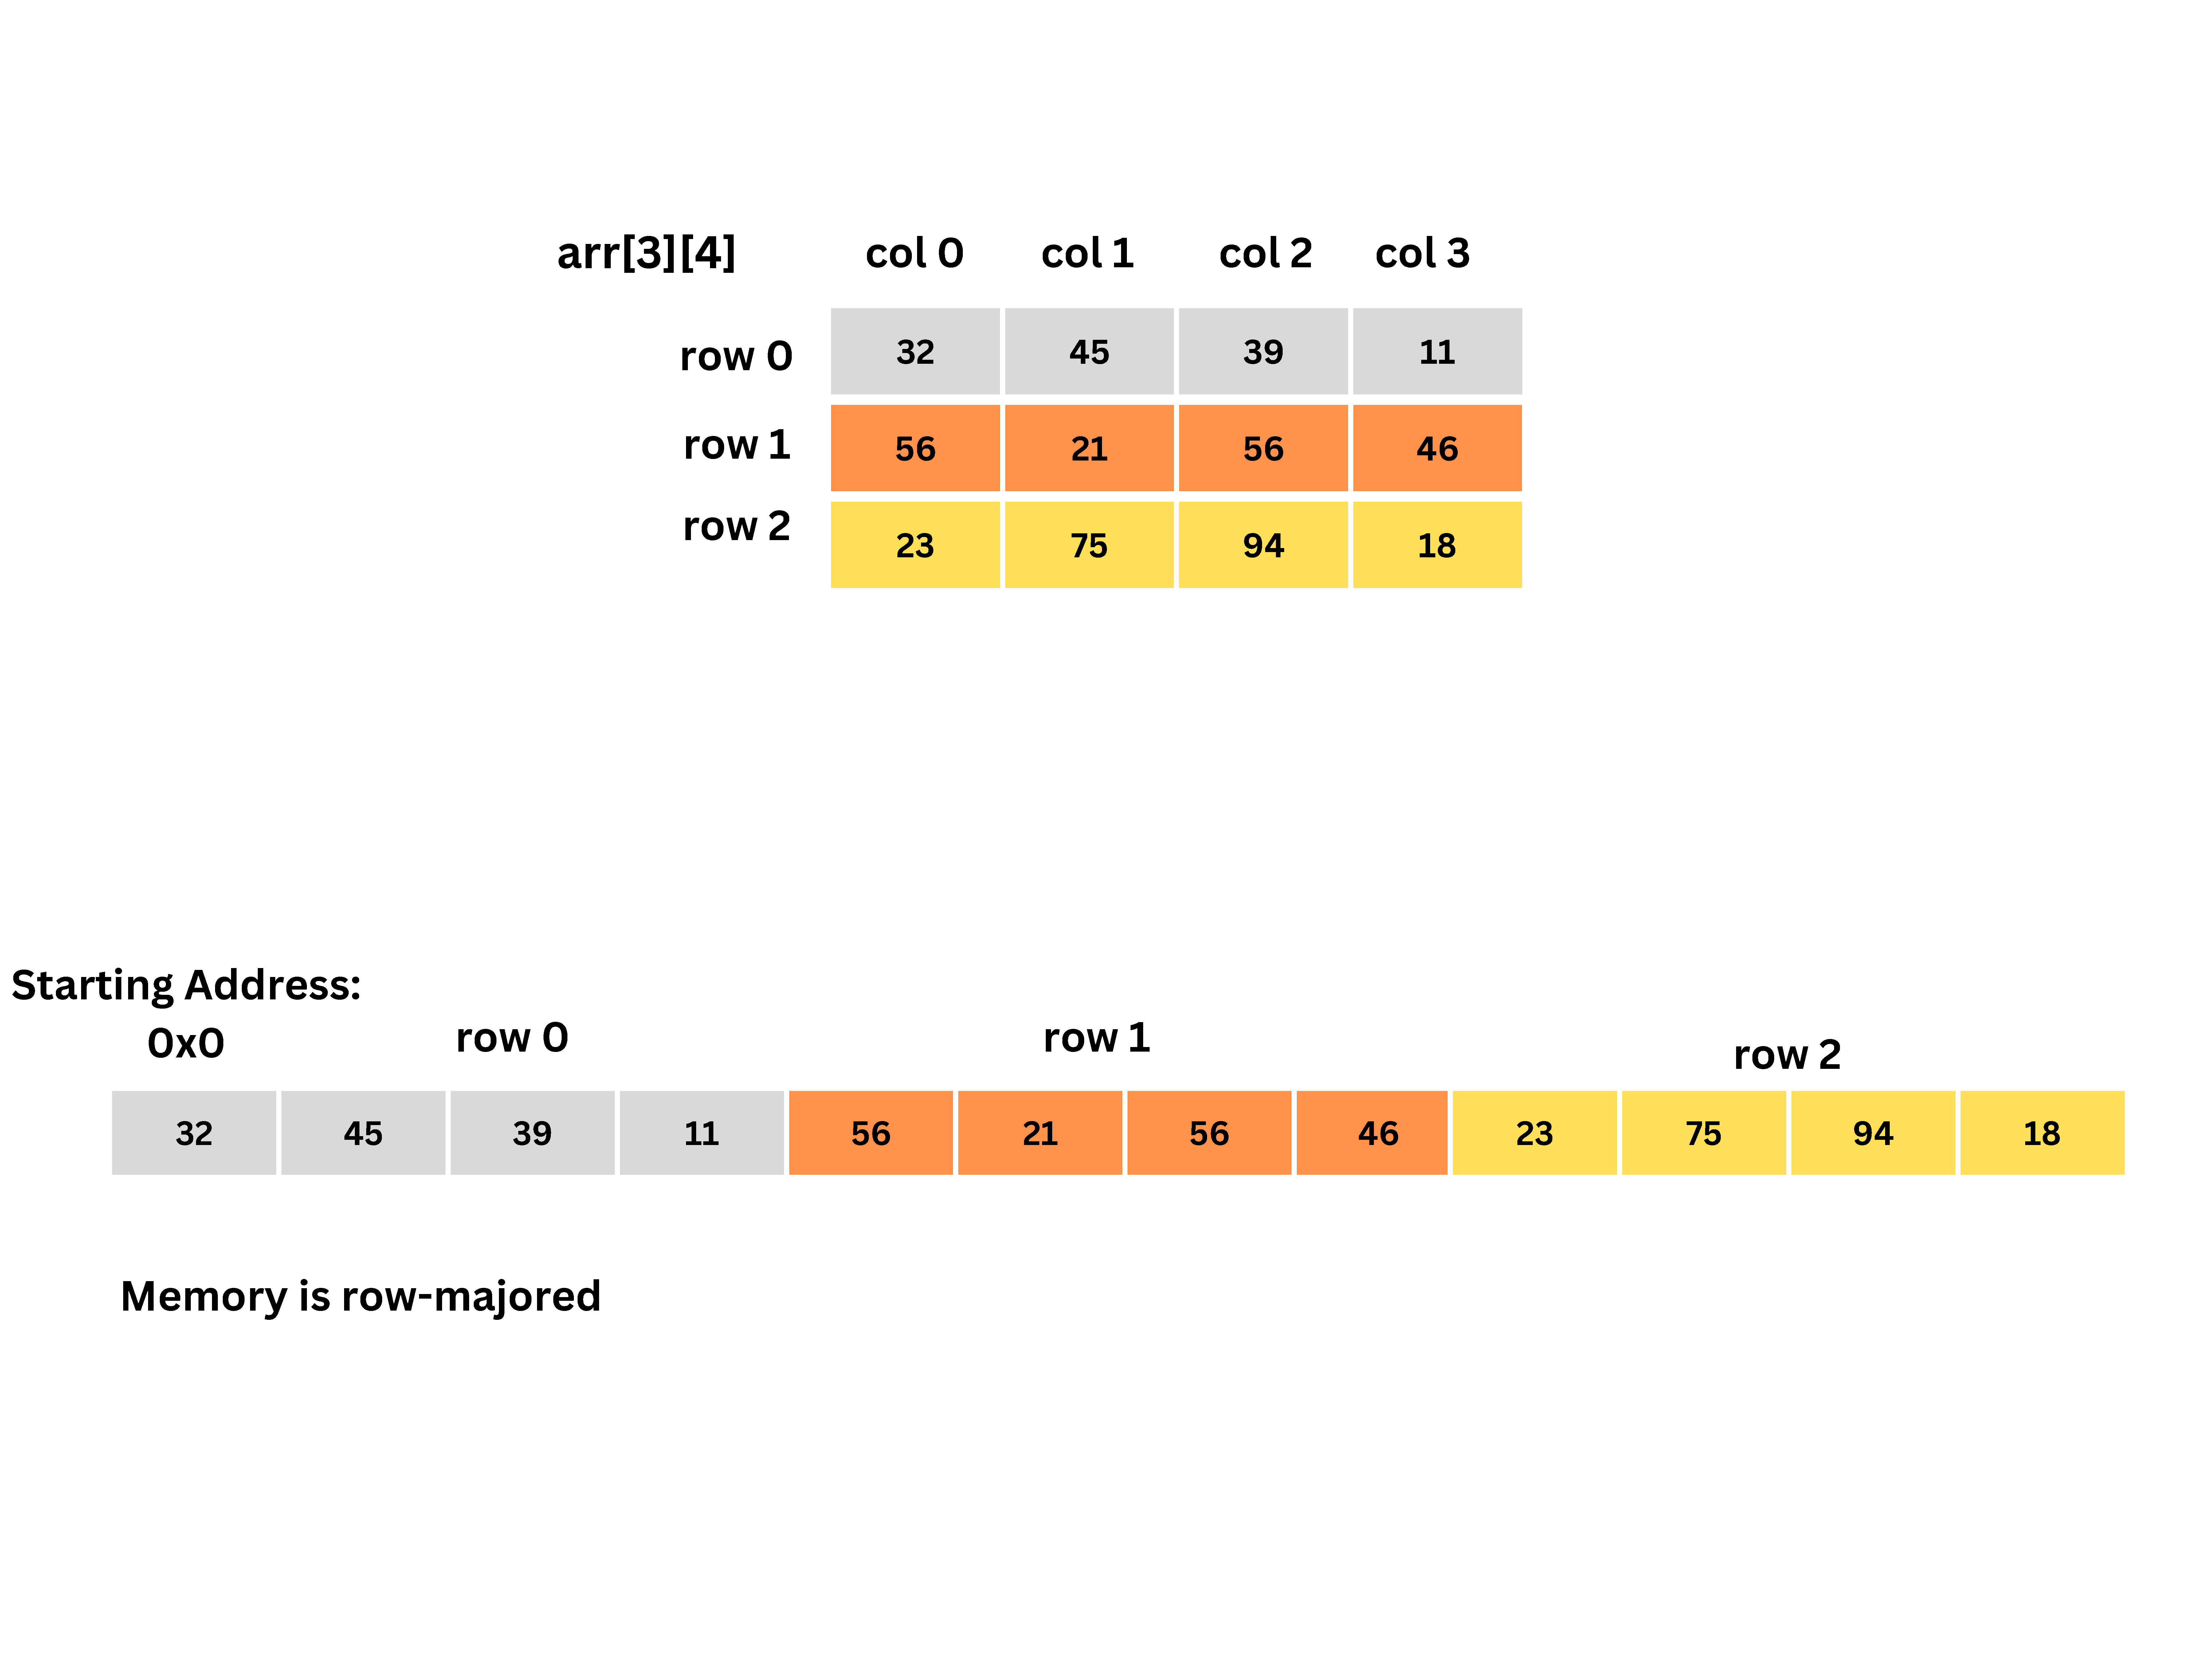
\includegraphics[width=\textwidth]{images/nested_arrays.pdf}
    \caption{Nested Array Diagram. In C, arrays are saved in \textit{row-major} order.}
    \label{fig:nested-array}
\end{figure}

\noindent Let us consider the array in Figure~\ref{fig:nested-array} as an example:  
Given the declaration:


\[
\texttt{char arr[3][4];}
\]

where \texttt{char} has \(\text{sizeof}(\texttt{char}) = 1\) byte, the memory address of \(\texttt{arr[1][2]}\) is:

\begin{align*}
    \text{arr}[2][3] &= \text{arr} + \text{sizeof}(\text{Type}) \times (C \times i + j) \\
    &= \text{arr} + 1 \times (4 \times 1 + 2) \\
    &= \text{arr} + 1 \times (4 + 2) \\
    &= \text{arr} + 6
\end{align*}


Thus, \(\texttt{arr[1][2]}\) is located 6 bytes after the base address \( arr \).
Since the array starts at address \texttt{0x0} from the figure, we need the element at address 6 which is 56. 

\noindent Let us consider another example, 

Given the declaration:

\[
\texttt{int arr[4][5];}
\]

where \texttt{int} has \(\text{sizeof}(\texttt{int}) = 4\) bytes, we want to find the equivalent \(\texttt{arr[i][j]}\) corresponding to \(\texttt{((int *)arr)[17]}\).

\(\texttt{((int *)arr)[17]}\) means that we cast our 2-D array, to one dimensional integer array. The memory offset of the \texttt{arr[17]} is \texttt{ 17 * sizeof(int)} which is 68. Remember, the equation above is used for the \textbf{memory address} of an element \( A[i][j] \) in a row-major order layout.

Now we can apply our equation:

\begin{align*}
arr[i][j] &= arr + \text{sizeof}(int) \times (C \times i + j) \\
        &= arr + 4 \times (5 \times i + j) \\
        &= arr + 20 \times i + 4 \times j \\
\end{align*}
Since the offset is 68 it means that \[
20 \times i + 4 \times j
\] 
must be equal to \texttt{68} we get \texttt{i = 3} and \texttt{j = 2} using through the following: 

\begin{align*}
20 \times i + 4 \times j &= 68
\end{align*}

Solving for \( i \):

\begin{align*}
i &= \frac{68}{20} = 3 \quad \text{(integer division)}
\end{align*}

Solving for \( j \):

\begin{align*}
j &= 68 \mod 20 = 4 \times j \\
  &=> 8 = 4 \times j \\
  &=> j = 2 \\
\end{align*}

Thus, the equivalent array access form is:
\[
\texttt{arr[3][2]}
\]

You may not need to memorize the equation. Once you understand how nested arrays are stored in \textit{row-major} order, as shown in Figure~\ref{fig:nested-array}, you can easily visualize the memory layout and determine the answer quickly. 

Using the equation is fine as long as you correctly implement \textit{pointer arithmetic} when necessary.

As examples of pointer arithmetic, consider the following declarations:

\begin{verbatim}
char    A[12];
char   *B[8];
int     C[6];
double *D[5];
\end{verbatim}

These declarations will generate arrays with the following parameters:
\begin{table}[h]
    \centering
    \begin{tabular}{c c c c c}
        \toprule
        \textbf{Array} & \textbf{Element size} & \textbf{Total size} & \textbf{Start address} & \textbf{Element i} \\ % <-- Added "\\" at the end
        \midrule
        A & 1  & 12  & \( x_A \)  & \( x_A + i \) \\ % <-- Added "\\" to separate rows
        B & 8  & 64  & \( x_B \)  & \( x_B + 8i \) \\ 
        C & 4  & 24  & \( x_C \)  & \( x_C + 4i \) \\ 
        D & 8  & 40  & \( x_D \)  & \( x_D + 8i \) \\ 
        \bottomrule
    \end{tabular}
\end{table}

\noindent\textbf{Related Problem 17} (Updated from Practice Problem 3.38) 
Based on the provided assembly code, find the values of \texttt{M} and \texttt{N} for the given C code below:
\begin{verbatim}
long P[M][N];
long Q[N][M];

long sum_element(long i, long j) {
    return P[i][j] + Q[j][i];
}
\end{verbatim}
The assembly code:
\begin{verbatim}
    sum_element:
        leaq    (%rdi,%rdi,2), %rdx
        addq    %rsi, %rdx
        leaq    (%rsi,%rsi,4), %rax
        addq    %rdi, %rax
        movq    Q(,%rax,8), %rax
        addq    P(,%rdx,8), %rax
        ret
\end{verbatim}

\texttt{M} is: \_\_\_ \newline
\texttt{N} is: \_\_\_ 

\textit{Answer: }\url{https://godbolt.org/z/68b4fEc38} 
\clearpage